
\chapter{Conference Information}


\section{Preface by the General Chair}

\begin{flushright}
August 25, 2015 
\par\end{flushright}

\noindent Welcome to the 2015 Conference on Empirical Methods in Natural
Language Processing. EMNLP is annually organized by SIGDAT, the Association
for Computational Linguistics' special interest group on linguistic
data and corpus-based approaches to NLP. This year the conference
will be held on September 17--21 in the enchanting city of Lisbon,
Portugal.\footnote{Conference website: \texttt{http://www.emnlp2015.org}}

EMNLP has continued to increase in prominence as one of the most important
conferences in Natural Language Processing (NLP). This year the conference
has experienced an unprecedented boost in submitted papers. I believe
that this reflects both the growth of the NLP field and also the health
and strength of the conference itself, with a history of many years
of solid work. With this level of interest at submission time, we
are also expecting a record attendance. The conference will span a
five-day period this year, and it requires a growing organization
structure.

Some of the features introduced in EMNLP 2014 will continue this year
(e.g., tutorials, new chairs, posters as parallel sessions, flat rates
and flexibility for tutorials and workshops, etc.). We also introduce
some innovations, like a revised selection process for which talks
are presented as talks versus posters.

This year I had the privilege of coordinating the conference from
my General Chair position. This has been a very instructive and enriching
exercise which showed me the conference as a whole, from many different
angles. Prefaces in the proceedings invariably praise the team of
organizers. This one will not be an exception. Organizing a large
conference as EMNLP requires excellent people working as a team in
multiple interrelated tasks. I have been lucky to work with an outstanding
team of people, from whom I learnt a lot. These aren't empty words.
I would like to thank each and every chair for the hard work that
made the conference a reality.

The Program Chairs, Jian Su and Chris Callison-Burch, did an excellent
job at putting together a very interesting program with over 300 papers.
They had to deal with a very large number of submissions, which exceeded
even our most optimistic expectations. As a consequence, they were
forced to be creative and to find solutions on the fly to adapt to
the situation. They recruited the largest ever program committee and
successfully managed a huge reviewing and decision making process
under a very tight schedule. A real gift for the general chair. They
complemented the program with very interesting keynote speakers, Yoshua
Bengio and Justin Grimmer who will present exciting research topics
for our community.

The EMNLP 2015 main conference is accompanied by 7 workshops and 8
tutorials during the first two days. The Workshops Chairs, Zornitsa
Kozareva and Jörg Tiedemann, and the Tutorials Chairs, Maggie Li and
Khalil Sima'an, conducted the selection processes in a joint effort
with the other ACL conferences in 2015 (NAACL and ACL-IJCNLP). This
has been the standard procedure from last years. It has the advantage
of starting early, avoiding duplicated reviewing and allowing a more
balanced selection among conferences. EMNLP attracted a varied and
interesting set of workshops and tutorials, which gives more value
to the conference.

Daniele Pighin and Yuval Marton were responsible for the always difficult
and sometimes thankless task of putting together the conference publications.
This is a very complex effort which involves coordination with almost
everyone in the team under the pressure of hard publication deadlines.
Yuval is serving in this position for a second year. Staggered two
year terms for publication chairs is a new addition for EMNLP starting
this year, and we hope that it will be a permanent feature. In the
first year, publication chairs will learn and do the bulk of proceedings
compilation. During the second year their role will be more advisory,
instructing and helping the first-year chair. This procedure will
help the transmission of the necessary know-how from year to year.
Thanks to Yuval and Daniele for accepting the challenge and making
it work wonderfully. Finally, this is the second year that EMNLP uses
a mobile app for the conference program (Conference4me). The publication
chairs also coordinated the integration of the app with SoftConf,
which is now smoother and more seamless.

The local organization team was led by André Martins and João Graça.
They did an amazing job, working hard and with all the complexities
and subtleties of local arrangements. One of the keys for the success
was the creation of a large team of local organizers with clearly
defined roles and responsibilities. They appointed very committed
people: Isabel Trancoso (Local Publicity Chair), Fernando Batista
(Handbook Chair), Bruno Martins (Website and App Chair), Luísa Coheur
(Student Volunteer Coordinator), and Helena Moniz (Local Arrangements
Chair). Thanks to all. I am especially pleased about the new website,
which was revamped and looks more professional everyday. This is certainly
a good investment for the future.

A large conference as EMNLP needs to focus on dissemination activities
too. Barbara Plank acted as the international Publicity Chair. She
did a fantastic job and coordinated very well with the local publicity
and the website chairs. The calls for papers, calls for participation,
and main news of the conference were timely distributed through ACL,
the usual distribution lists, and also through the conference website
and two Facebook and Twitter accounts. The EMNLP2015 Twitter account
garnered more followers than in previous years.

I am really grateful to SIGDAT. Its secretary, Noah Smith, acted as
the liasion between SIGDAT and the conference organizers. He was always
available and ready to help with very good advice. SIGDAT also provided
the funds for the student scholarship program. These grants help covering
traveling expenses to a dozen of students. The committee appointed
for collecting the applications and making the decisions was formed
by Francisco Guzmán and Llu\'{i}s Padró, who had to analyze all the
information and decide the awardees in only a few days.

Another sign of the health of EMNLP and the field in general is the
interest showed by sponsors. Thanks to the work of our sponsorship
team, formed by João Graça and Hang Li, in coordination with the ACL
International Sponsorship Committee, we got a record number of 13
sponsors for EMNLP 2015 (2 platinum, 3 gold, 6 silver and 2 bronze).
In addition to these direct sponsors, we also have several smaller
supporters, exhibitors, and institutional partners. We are extremely
grateful to all these companies and institutions, which make a better
conference possible at a more affordable registration fee.

Additionally, we counted on the invaluable help of Priscilla Rasmussen,
supporting the local organization in all fronts with her broad experience.
She took care of the registration process too. We also got very good
advice, know-how, and helpful software and forms from last year general
chair and local organizers, Alessandro Moschitti and Kareem Darwish.
Thank you.

Finally, I would like to thank the authors of submitted and accepted
papers, and all the attendees to the conference, who will be the main
actors from September 17 to September 21, 2015. I am convinced that
we will experience a fantastic conference, scientifically exciting
and full of fond memories, in the unique environment of Lisbon. 

\begin{flushright}
\emph{Lluís Màrquez}\index{Màrquez, Lluís}\\
 EMNLP 2015 General Chair 
\par\end{flushright}

\newpage{}


\section{Preface by the Program Committee Co-Chairs}

\begin{flushright}
August 25, 2015 
\par\end{flushright}

\noindent Welcome to the 2015 Conference on Empirical Methods in Natural
Language Processing! This year we received a record number of submissions.
There were 1300 valid submissions. The 600 long papers and 700 short
papers were allocated to one of 15 areas. The most popular areas this
year were Semantics, Statistical Models and Machine Learning Methods,
Text Mining and NLP applications, and Machine Translation.

Reviewing for a conference this size involves an enormous volunteer
effort from many individuals. We are very grateful to our 30 area
chairs and to the more than 900 researchers who reviewed the submissions.
We accepted 312 papers (157 long and 155 short papers), representing
a global acceptance rate of 24\%. An additional 17 papers accepted
by the TACL journal were presented at the conference as well.

To decide whether the accepted papers should be presented as talks
or posters, we asked the area chairs, the reviewers, and the authors
of accepted papers to vote on which papers they would like to attend.
We showed the title of each paper and its abstract, but not its authors.
400 people provided their input. We selected talks based on popularity,
while ensuring that each area was represented by at least one session.
Our rationale for taking a vote was that papers that many people wanted
to attend would be better served by presenting a talk in a large room,
while papers with more specialized interest would benefit from the
one-on-one interactions facilitated by posters. Rather than doing
large plenary poster sessions, we have scheduled two parallel poster
sessions with small batches of thematically similar papers that will
be run simultaneously with the talks.

We selected best papers from a shortlist of 20 papers that were nominated
by the area chairs. The best paper committee ranked the nominees,
and based on their rankings we selected the following papers for the
best paper awards: 
\begin{itemize}[itemsep=0pt]
\item Best paper - \textit{Broad-coverage CCG Semantic Parsing with AMR}
by Yoav Artzi, Kenton Lee and Luke Zettlemoyer. 
\item Best paper - \textit{Semantically Conditioned LSTM-based Natural Language
Generation for Spoken Dialogue Systems} by Tsung-Hsien Wen, Milica
Gasic, Nikola Mrkšić, Pei-Hao Su, David Vandyke and Steve Young.
\end{itemize}
IBM has provided a cash scholarship for us to award to the best student
paper. This will go to Tsung-Hsien Wen, since he is currently a student.
The following papers received an honorable mention for the best paper
award: 
\begin{itemize}[itemsep=0pt]
\item Honorable mention for best paper - \textit{Traversing Knowledge Graphs
in Vector Space} by Kelvin Guu, John Miller and Percy Liang. 
\item Honorable mention for best paper - \textit{Building a shared world:
mapping distributional to model-theoretic semantic spaces} by Aurélie
Herbelot and Eva Maria Vecchi. 
\item Honorable mention for best paper - \textit{Language Understanding
for Text-based Games using Deep Reinforcement Learning } by Karthik
Narasimhan, Tejas Kulkarni and Regina Barzilay. 
\item Honorable mention for best short paper - \textit{Joint Lemmatization
and Morphological Tagging with Lemming} by Thomas Müller, Ryan Cotterell,
Alexander Fraser and Hinrich Schütze. 
\item Honorable mention for best short paper - \textit{Semi-Supervised Bootstrapping
of Relationship Extractors with Distributional Semantics} by David
S. Batista, Bruno Martins and Mário J. Silva.
\end{itemize}
This year we created a new ``Best data set or resource'' award,
since so much work in our community is driven by data. The paper that
receiving this inaugural distinction is: 
\begin{itemize}[itemsep=0pt]
\item Best data set or resource - \textit{A large annotated corpus for
learning natural language inference} by Samuel R. Bowman, Gabor Angeli,
Christopher Potts and Christopher D. Manning.
\end{itemize}
With two honorable mentions: 
\begin{itemize}[itemsep=0pt]
\item Notable data set or resource - \textit{That's So Annoying!!!: A Lexical
and Frame-Semantic Embedding Based Data Augmentation Approach to Automatic
Categorization of Annoying Behaviors using \#petpeeve Tweets} by William
Yang Wang and Diyi Yang. 
\item Notable data set or resource - \textit{Modeling Reportable Events
as Turning Points in Narrative} by Jessica Ouyang and Kathy McKeown.
\end{itemize}
We decided to give more awards than in past years by recognizing papers
with honorable mentions and by creating the new best data or resource
award. Our goal was to recognize roughly the top 1\% of all of the
submissions to the conference with awards (recognizing approximately
the top 5\% of accepted papers). We are very grateful to our invited
speakers Yoshua Bengio and Justin Grimmer.

Yoshua Bengio is professor of Computer Science and Operations Research
at the Université de Montréal. He is the author of two books and more
than 200 publications, the most cited being in the areas of deep learning,
recurrent neural networks, probabilistic learning algorithms, natural
language processing and manifold learning. He co-directs the Canadian
Institute for Advanced Research's program on deep learning. He is
on the board of NIPS. Professor Bengio's research into deep learning
has had a dramatic impact on the field of NLP in the past few years,
and has invigorated interest in AI through machine learning.

Justin Grimmer is an associate professor of Political Science at Stanford
University. His research uses statistical methods to examine American
politics. He is the author of two books on the topic ``Representational
Style in Congress: What Legislators Say and Why It Matters'' and
``The Impression of Influence: How Legislator Communication and Government
Spending Cultivate a Personal Vote.'' His work has appeared in the
American Political Science Review, American Journal of Political Science,
Journal of Politics, Political Analysis, Proceedings of the National
Academy of Sciences, Regulation and Governance, and Poetics. Professor
Grimmer's research points to exciting new directions for computational
social science and how the field of NLP can facilitate research in
many areas.

We thank them in advance for coming to the conference and sharing
their insights.

We would also like to thank our general chair Lluís Màrquez, André
Martins and João Graça and colleagues for their excellent work with
the local organization, and Yuval Marton and Daniele Pighin for doing
an excellent job assembling these proceedings.

We thank SIGDAT for inviting us to serve as Program Co-Chairs of EMNLP
2015. We hope that the conference is an excellent one. Enjoy your
stay in Lisbon! 

\begin{flushright}
\emph{Chris Callison-Burch and Jian Su} \index{Callison-Burch, Chris}\index{Su, Jian}
\\
 EMNLP 2015 Program Committee Co-Chairs 
\par\end{flushright}

\clearpage{}


\section{Conference Committee}
\begin{itemize}[itemsep=7pt, leftmargin=0cm, label={}]
\item \textbf{General Chair}

\begin{itemize}[nosep, leftmargin=0.5cm, label={}]
\item Lluís Màrquez, Qatar Computing Research Institute\index{Màrquez, Lluís}
\end{itemize}
\item \textbf{Program co-Chairs}

\begin{itemize}[nosep, leftmargin=0.5cm, label={}]
\item Chris Callison-Burch, University of Pennsylvania \index{Callison-Burch, Chris}
\item Jian Su, Institute for Infocomm Research (I2R) \index{Su, Jian}
\end{itemize}
\item \textbf{Workshops co-Chairs}

\begin{itemize}[nosep, leftmargin=0.5cm, label={}]
\item Zornitsa Kozareva, Yahoo! Labs\index{Kozareva, Zornitsa}
\item Jörg Tiedemann, University of Helsinki\index{Tiedemann, Jörg}
\end{itemize}
\item \textbf{Tutorial co-Chairs}

\begin{itemize}[nosep, leftmargin=0.5cm, label={}]
\item Maggie Li, Hong Kong Polytechnic University \index{Li, Maggie}
\item Khalil Sima'an, University of Amsterdam \index{Sima'an, Khalil}
\end{itemize}
\item \textbf{Publication co-Chairs} 

\begin{itemize}[nosep, leftmargin=0.5cm, label={}]
\item Daniele Pighin, Google Inc. \index{Pighin, Daniele} 
\item Yuval Marton, Microsoft Corp. \index{Marton, Yuval}
\end{itemize}
\item \textbf{Publicity Chair} 

\begin{itemize}[nosep, leftmargin=0.5cm, label={}]
\item Barbara Plank, University of Copenhagen \index{Plank, Barbara}
\end{itemize}
\item \textbf{Sponsorship Team}

\begin{itemize}[nosep, leftmargin=0.5cm, label={}]
\item João Graça, Unbabel Inc. \index{Graça, João}
\item Hang Li, Huawei Technologies (ISC Representative for EMNLP) \index{Li, Hang}
\end{itemize}
\item \textbf{Student Scholarship co-Chairs}

\begin{itemize}[nosep, leftmargin=0.5cm, label={}]
\item Fancisco Guzmán, Qatar Computing Research Institute\index{Guzmán, Fanciscog}
\item Lluís Padró, Technical University of Catalonia\index{Padró, Lluís}
\end{itemize}
\item \textbf{SIGDAT Liaison}

\begin{itemize}[nosep, leftmargin=0.5cm, label={}]
\item Noah Smith, University of Washington\index{Smith, Noah A.}
\end{itemize}
\item \textbf{Local co-Chairs}

\begin{itemize}[nosep, leftmargin=0.5cm, label={}]
\item André Martins, Priberam \index{Martins, André}
\item João Graça, Unbabel Inc. \index{Graça, João}
\end{itemize}
\item \textbf{Program co-Chairs}

\begin{itemize}[nosep, leftmargin=0.5cm, label={}]
\item Chris Callison-Burch, University of Pennsylvania\index{Callison-Burch, Chris}
\item Jian Su, Institute for Infocomm Research (I2R)\index{Su, Jian}
\end{itemize}
\item \textbf{Area Chairs}

\begin{itemize}[leftmargin=0.5cm, itemsep=6pt, label={}]
\item \emph{Computational Psycholinguistics}

\begin{itemize}[nosep, leftmargin=0.5cm, label={}]
\item Vera Demberg, Saarland University\index{Demberg, Vera}
\end{itemize}
\item \emph{Discourse, Dialogue, and Pragmatics}

\begin{itemize}[nosep, leftmargin=0.5cm, label={}]
\item Kentaro Inui, Tohoku University\index{Inui, Kentaro}
\item Oliver Lemon, Heriot Watt University\index{Lemon, Oliver}
\end{itemize}
\item \emph{Information Extraction}

\begin{itemize}[nosep, leftmargin=0.5cm, label={}]
\item Heng Ji, Rensselaer Polytechnic Institute\index{Ji, Heng}
\item Sebastian Riedel, University College London\index{Riedel, Sebastian}
\item Jing Jiang, Singapore Management University\index{Jiang, Jing}
\end{itemize}
\item \emph{Information Retrieval and Question Answering}

\begin{itemize}[nosep, leftmargin=0.5cm, label={}]
\item Zhu Xiaoyan, Tsinghua University\index{Xiaoyan, Zhu}
\item Liu Ting, Harbin Institute of Technology\index{Ting, Liu}
\end{itemize}
\item \emph{Language and Vision}

\begin{itemize}[nosep, leftmargin=0.5cm, label={}]
\item Julia Hockenmaier, University of Illinois Urbana Champaign\index{Hockenmaier, Julia}
\end{itemize}
\item \emph{Machine Translation and Multilinguality}

\begin{itemize}[nosep, leftmargin=0.5cm, label={}]
\item Zhang Min, SooChow University\index{Min, Zhang}
\item Lucia Specia, University of Sheffield\index{Specia, Lucia}
\item Marine Carput, University of Maryland\index{Carput, Marine}
\end{itemize}
\item \emph{NLP for the Web and Social Media, including Computational Social
Science}

\begin{itemize}[nosep, leftmargin=0.5cm, label={}]
\item Alice Oh, KAIST\index{Oh, Alice}
\item Brendan O'Connor, University of Massachusetts Amherst\index{O'Connor, Brendan}
\end{itemize}
\item \emph{Phonology, Morphology, and Word Segmentation}

\begin{itemize}[nosep, leftmargin=0.5cm, label={}]
\item Greg Kondrak, University of Alberta\index{Kondrak, Greg}
\item Xu Sun, Peking University\index{Sun, Xu}
\end{itemize}
\item \emph{Semantics}

\begin{itemize}[nosep, leftmargin=0.5cm, label={}]
\item Marco Baroni, University of Trento\index{Baroni, Marco}
\item Shiqi Zhao, Baidu\index{Zhao, Shiqi}
\item Percy Liang, Stanford University\index{Liang, Percy}
\end{itemize}
\item \emph{Sentiment Analysis and Opinion Mining}

\begin{itemize}[nosep, leftmargin=0.5cm, label={}]
\item Ku Lun-Wei, Institute of Information Science, Academia Sinica\index{Lun-Wei, Ku}
\item He Yulan, Aston University\index{Yulan, He}
\end{itemize}
\item \emph{Spoken Language Processing}

\begin{itemize}[nosep, leftmargin=0.5cm, label={}]
\item Mari Ostendorf, University of Washington\index{Ostendorf, Mari}
\end{itemize}
\item \emph{Statistical Models and Machine Learning Methods}

\begin{itemize}[nosep, leftmargin=0.5cm, label={}]
\item Trevor Cohn, University of Melbourne\index{Cohn, Trevor}
\item Jordan Boyd-Graber, University of Colorado\index{Boyd-Graber, Jordan}
\end{itemize}
\item \emph{Summarization and Generation}

\begin{itemize}[nosep, leftmargin=0.5cm, label={}]
\item Meg Mitchell, Microsoft Research\index{Mitchell, Meg}
\item Furu Wei, Microsoft Research Asia\index{Wei, Furu}
\end{itemize}
\item \emph{Tagging, Chunking, Syntax and Parsing}

\begin{itemize}[nosep, leftmargin=0.5cm, label={}]
\item Shay Cohen, University of Edinburgh\index{Cohen, Shay}
\item Yue Zhang, Singapore University of Technology and Design\index{Zhang, Yue}
\item Yusuke Miyao, National Institute of Informatics, Japan\index{Miyao, Yusuke}
\end{itemize}
\item \emph{Text Mining and NLP applications}

\begin{itemize}[nosep, leftmargin=0.5cm, label={}]
\item Sophia Ananiadou, University of Manchester\index{Ananiadou, Sophia}
\end{itemize}
\end{itemize}
\item \textbf{Local Organization Committee}

\begin{itemize}[itemsep=6pt, leftmargin=0.2cm, label={}]
\item \textit{Local co-Chairs} 

\begin{itemize}[nosep, leftmargin=0.5cm, label={}]
\item André Martins, Priberam \index{Martins, André}
\item João Graça, Unbabel Inc. \index{Graça, João}
\end{itemize}
\item \emph{Local Arrangements Chair}

\begin{itemize}[nosep, leftmargin=0.5cm, label={}]
\item Helena Moniz, University of Lisbon \& INESC-ID \index{Moniz, Helena}
\end{itemize}
\item \textit{Local Publicity Chair}

\begin{itemize}[nosep, leftmargin=0.5cm, label={}]
\item Isabel Trancoso, University of Lisbon\index{Trancoso, Isabel}
\end{itemize}
\item \textit{Conference Handbook Chair} 

\begin{itemize}[nosep, leftmargin=0.5cm, label={}]
\item Fernando Batista, University Institute of Lisbon (ISCTE-IUL) \index{Batista, Fernando}
\end{itemize}
\item \textit{Website and App Chair} 

\begin{itemize}[nosep, leftmargin=0.5cm, label={}]
\item Bruno Martins, University of Lisbon \index{Martins, Bruno}
\end{itemize}
\item \emph{Student Volunteer Coordinator}

\begin{itemize}[nosep, leftmargin=0.5cm, label={}]
\item Luísa Coheur, University of Lisbon\index{Coheur, Luísa}
\end{itemize}
\end{itemize}
\end{itemize}
\clearpage{}


\section{Social events}

\noindent EMNLP 2015 will feature welcome and farewell receptions,
respectively on the 18th of September (second day of the conference)
and on the 21st of September (the last day of the conference). These
receptions will take place at Culturgest, the main conference venue.
EMNLP 2015 will also feature a conference dinner, on Sunday the 20th
of September, which will take place at Páteo Alfacinha, in the Ajuda
area of Lisbon. Transportation to Páteo Alfacinha will be arranged.

\begin{center}
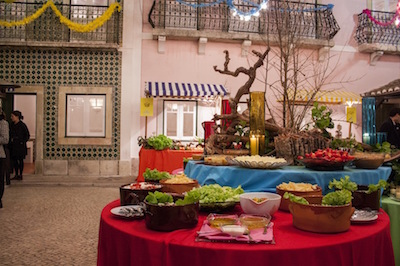
\includegraphics[height=3cm]{content/images-web/dinner-pateo-jantar-arraial}\ 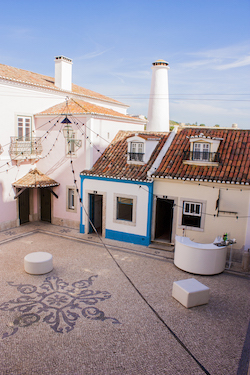
\includegraphics[height=3cm]{content/images-web/dinner-pateo-exterior}\ 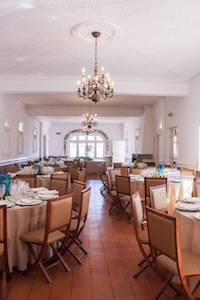
\includegraphics[height=3cm]{content/images-web/dinner-pateo-sala}
\par\end{center}

Páteo Alfacinha was created in 1981, featuring several spaces typical
from the beginning of XX century Lisbon: a chapel, a barber shop,
a tavern, a bakery, a pub, an antiquary, and houses for the “alfacinhas”
(inhabitants of Lisbon). Nowadays, Páteo Alfacinha remains a multifaceted
place, with restaurants and facilities for events such as EMNLP's
conference dinner.


\subsection*{Welcome Reception}

Friday, September 18th at 18:30 at Culturgest


\subsection*{Conference Dinner}

Sunday, September 20th at 19:00 at Pateo Alfacinha

First buses depart from Culturgest at 18:15. 

Last returning bus depart from Páteo Alfacinha at 24:00.


\subsection*{Farewell Drink}

Monday, September 21th at 18:30 at Culturgest
